\documentclass[./GL2017.tex]{subfiles}\providecommand{\econtexRoot}{}
\renewcommand{\econtexRoot}{.}

% Different execution depending on whether compiling main file or as standalone subfile
\onlyinsubfile{\externaldocument{GL2017}} % Get xrefs -- esp to appendix 
%-- from main file; only works properly if main file has already been compiled; 
%order: Compile this file, then main, then this one again
\begin{document}

\hfill{\tiny \texname.tex, \today}

\begin{verbatimwrite}{GL2017.title}  % Write title to .title file
Guerrieri and Lorenzoni (2017) REMARK
\end{verbatimwrite}

\title{Guerrieri and Lorenzoni (2017) \\ REMARK}

\author{William Du \and Tung-Sheng Hsieh}

\keywords{Credit Crises, Precautionary Savings, Liquidity Trap, Replication}

\maketitle 

\hypertarget{abstract}{}
\begin{abstract}
This paper uses the Econ-ARK/HARK toolkit to replicate the results of Guerrieri and Lorenzoni (2017). We create a new AgentType, GLConsumerType, that inherits the IndShockConsumerType and a Solver, GLSolver, that inherits the ConsIndShockSolver. We managed to closely replicate the initial Optimal Consumption and Labor Supply Steady States found Figure 1 of the paper. 


\end{abstract}


\begin{authorsinfo}
\name{Contact: \href{mailto:wdu9@jhu.edu}{\texttt{wdu9@jhu.edu}}, \href{mailto:thsieh11@jhu.edu}{\texttt{thsieh11@jhu.edu}}, Department of Economics, 590 Wyman Hall, Johns Hopkins University, Baltimore, MD 21218}
\end{authorsinfo}

\titlepagefinish

\newtheorem{defn}{Definition}
\newtheorem{theorem}{Theorem}

\hypertarget{Summary}{}
\section{Summary}

This paper uses a heterogeneous agents model with incomplete markets and endogenous labor supply to analyze the effects of a credit crunch on consumer spending. 

Main Findings: 

(i) A credit crunch leads to a fall in consumption and real interest rates due to a forced deleveraging and an increase in precautionary savings.

(ii) Adding nominal rigidities to the baseline model may  exacerbate the effects on output as the zero lower bound may prevent the real interest rate from falling sufficiently in order to attain the flexible price equilibrium.

(iii) Adding durable goods to the baseline model does not fundamentally alter the baseline result mentioned in (i). In this extension, there is a fall in consumption in both non durables and durables for credit constrained consumers and an increase in precautionary savings through durables and bonds for net lenders.  

\hypertarget{Non-Technical Overview}{}
\section{Non-Technical Overview}

The authors consider a heterogeneous agents model where there is a continuum of infinitely lived households with idiosyncratic uncertainty to their labor productivity and subject to a borrowing limit.  In order to understand the effects of a credit crunch, the authors analyze how a shock to the borrowing limit (a tightening in credit) influences each household's consumption decision and the resulting interest rate dynamics. 

\subsection{Baseline Model}
\begin{itemize}
\item{Households/Producers}\\
There is a continuum of infinitely lived households with preferences represented by
the utility function:
\begin{verbatimwrite}{\EqDir/Equation1.tex}
	\begin{align}
		\mathrm{E}\left[\sum_{t=0}^{\infty} \beta^{t} U\left(c_{i t}, n_{i t}\right)\right]\\
		U(c, n)=\frac{c^{1-\gamma}}{1-\gamma}+\psi \frac{(1-n)^{1-\eta}}{1-\eta}
	\end{align}
\end{verbatimwrite}
	\begin{align}
		\mathrm{E}\left[\sum_{t=0}^{\infty} \beta^{t} U\left(c_{i t}, n_{i t}\right)\right]\\
		U(c, n)=\frac{c^{1-\gamma}}{1-\gamma}+\psi \frac{(1-n)^{1-\eta}}{1-\eta}
	\end{align}


Each household chooses $c_{it}$ and $n_{it}$ to maximize their lifetime expected utility  subject to their household budget constraint described below. Production is dependent on the choice of $n_{it}$
\begin{equation}
y_{i t}=\theta_{i t} n_{i t}
\end{equation}

where $ \theta_{i t}$ is an idiosyncratic shock to the labor productivity of  household, which follows a Markov chain on the space $\left\{\theta^{1}, \ldots, \theta^{S}\right\}$. Let $\theta^{1} =0$.

\item{Household Budget Constraint}\\

\begin{equation}
q_{t} b_{i t+1} +c_{i t}+\tilde{\tau}_{i t} \leq b_{i t}+y_{i t}
\end{equation}


where $q_{t}$ is the bond price, $\tilde{\tau}_{i t}$ are taxes such that $\tilde{\tau}_{i t}=\tau_{t}$ if $\theta_{i t}>0$ and $\tilde{\tau}_{i t}=\tau_{t}-v_{t}$ if $\theta_{i t}=0$ where $v_{t}$ is unemployment insurance. $b_{i t+1}$ are bond holdings.

Household debt is bounded below by an exogenous limit $\phi > 0$. That is,
\begin{equation}
b_{i t+1} \geq-\phi
\end{equation}

A credit crunch is equivalent to lowering the value of $\phi$.

\item{Government}\\
The government chooses the aggregate supply of bonds $B_{t}$, the unemployment benefit $v_{t}$ and the lump sum tax $\tau_{t}$ so as to satisfy the budget constraint
\begin{equation}
B_{t}+v_{t} u=q_{t} B_{t+1}+\tau_{t}
\end{equation}

where where u = Pr ($\theta_{it}$ = 0) is the fraction of unemployed agents in the population.

We assume that the supply of government bonds $B$ and unemployment insurance $v$ are kept constant.
Taxes $\tau$ adjust to ensure the government budget balances.


\end{itemize}



\subsection{Dynamic Program}

For household i, the Bellman equation is


\begin{align}
V_{it}(b_{it}, \theta_{it})=\max _{c_{it}, n_{it}, b_{it+1}} U(c_{it}, n_{it})+\beta E\left[V\left(b_{it+1}, \theta_{it+1}\right) \mid \theta_{it}\right] \\
\text { s.t. }  b_{it}+\theta_{it} n_{it} -\tau(\theta_{it}) \geq q_{t} b_{it+1}+c_{it}, \\
b_{it+1}+\phi \geq 0
\end{align}

\subsection{Results}
\begin{itemize}
\item{Baseline Model}\\
Consumers who's borrowing constraint was slack are forced to deleverage when the borrowing limit falls. These consumers both increase their labor supply and reduce their consumption. Furthermore, this deleveraging requires in an increase in  the demand for bonds to a fall in the real interest rate.

There is an increase in precautionary savings for non-constrained consumers (who are not at the right tail of the initial bond distribution) in order to buffer themselves against future shocks. Increasing their precautionary motive requires an increase in the demand for bonds leading the real interest rate to fall.

Only highly productive consumers (those who did not experience a significant negative productivity shock) will decumulate bonds and increase consumption from lowered interest rates.

\end{itemize}


\hypertarget{Replication}{}
\section{Replication}

\begin{table}
\begin{center}\renewcommand{\arraystretch}{1.5}
\caption{Microeconomic Model Calibration}\label{table:Calibration}
\begin{tabular}{|c|ccl|c|}
\hline
\multicolumn{5}{|l|}{Calibrated Parameters}  \\ \hline
Description                     & \multicolumn{1}{c}{Parameter} & Value & \multicolumn{2}{c|}{Source}\\ \hline
Permanent Income Growth Factor  & \multicolumn{1}{c}{$\PGro$} & 1.03 & \multicolumn{2}{c|}{PSID: Carroll (1992)} \\
Interest Factor                 & \multicolumn{1}{c}{$\Rfree$} & 1.04 & \multicolumn{2}{c|}{Conventional} \\
Time Preference Factor          & \multicolumn{1}{c}{$\beta$} & 0.96 & \multicolumn{2}{c|}{Conventional} \\
Coefficient of Relative Risk Aversion & \multicolumn{1}{c}{$\CRRA$} & 2 & \multicolumn{2}{c|}{Conventional} \\
Probability of Zero Income      & \multicolumn{1}{c}{$\pZero$} & 0.005 & \multicolumn{2}{c|}{PSID: Carroll (1992)} \\
Std Dev of Log Permanent Shock  & \multicolumn{1}{c}{$\sigma_{\pshk}$} & 0.1 & \multicolumn{2}{c|}{PSID: Carroll (1992)} \\
Std Dev of Log Transitory Shock & \multicolumn{1}{c}{$\sigma_{\theta}$} & 0.1 & \multicolumn{2}{c|}{PSID: Carroll (1992)} \\ \hline
\end{tabular}
\end{center}
\end{table}
\begin{table}
\begin{center}\renewcommand{\arraystretch}{1.5}
\caption{Model Characteristics Calculated from Parameters}\label{table:Calibration}
\begin{tabular}{|c|ccl|c|}
\hline
%\multicolumn{5}{|l|}{Model Characteristics Calculated From Parameters}  \\ \hline
                                            & \multicolumn{3}{c|}{}                                      & Approximate \\
                                            & \multicolumn{3}{c|}{}                                       & Calculated \\
Description                                 & \multicolumn{3}{c|}{Symbol and Formula}                       & Value \\ \hline
Finite Human Wealth Measure                 & $\Rnorm^{-1}$ & $\equiv$ & $\PGro/\Rfree$                    & 0.990 \\
PF Finite Value of Autarky Measure& $\beth$ & $\equiv$ & $\beta \PGro^{1-\CRRA}$                    & 0.932 \\
Growth Compensated Permanent Shock            & $\InvEpShkInv $ & $\equiv$ & $ (\EpShkInv)^{-1}$               & 0.990 \\
Uncertainty-Adjusted Growth                 & $\PGroAdj $ & $\equiv$ & $ \PGro \InvEpShkInv$        & 1.020 \\
Utility Compensated Permanent Shock                & $\uInvEpShkuInv $ & $\equiv$ & $ (\Ex_{t}[\pShk^{1-\CRRA}])^{1/(1-\CRRA)}$ & 0.990 \\
Utility Compensated Growth                     & $\PGrouAdj $ & $\equiv$ & $ \PGro \uInvEpShkuInv$        & 1.020 \\
Absolute Patience Factor                    & $\Pat_{\phantom{\Rfree}} $ & $\equiv$ & $ (\Rfree \beta)^{1/\CRRA}$                & 0.999 \\
Return Patience Factor                      & $\PatR$ & $\equiv$ & $\Pat/\Rfree $     & 0.961 \\
PF Growth Patience Factor    & $\PatPGro$ & $\equiv$ & $\Pat/\PGro $      & 0.970 \\
Growth Patience Factor                      & $\PatPGroAdj$ & $\equiv$ & $ \Pat/\PGroAdj$& 0.980 \\
Finite Value of Autarky Measure         & $\DiscAltuAdj $ & $\equiv$ & $ \beta \PGro^{1-\CRRA}\uInvEpShkuInv^{1-\CRRA}$       & 0.941 \\ \hline
\end{tabular}
\end{center}
\end{table}


The wage process is approximated by a 12-state Markov chain, following the approach in Tauchen (1986).
Since the GLConsumerType is a subclass of the IndShockConsumerType , we must specify an income distribution. 
However, because there are no transitory nor permanent shocks to income in the model, the Income distribution is degenerate. 

\subsection{Initial Steady States }
See Figure \ref{fig:Figure1} and Figure \ref{fig:Figure2} for consumption and labor supply functions for $ \theta_{it} = \theta^{2} , \theta^{8}$ from out replication codes.

\begin{figure}
\centerline{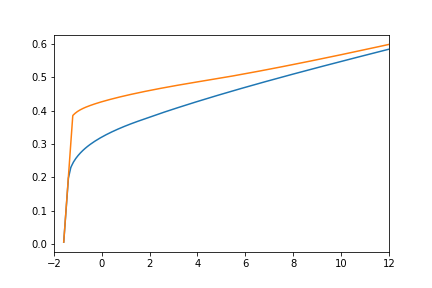
\includegraphics[width=6in]{Figures/Figure1.png}}
\label{fig:Figure1}
\caption{Consumption Functions for  $ \theta_{it} = \theta^{2} , \theta^{8}$}
\centerline{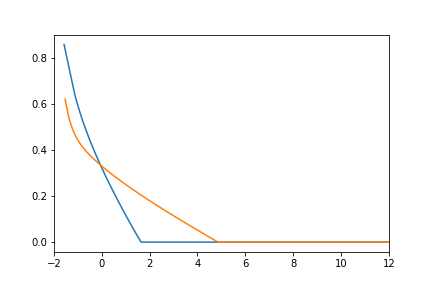
\includegraphics[width=6in]{Figures/Figure2.png}}
\label{fig:Figure2}
\caption{Labor Supply Functions for $ \theta_{it} = \theta^{2} , \theta^{8}$}
\end{figure}

It is apparent that consumption varies with bond holdings.  At high levels of bond holdings, the consumer's behavior is similar to that of the Permanent Income Hypothesis. The consumption function is concave due to the precautionary motive as there is positive probability that the agent will be unemployed. The labor supply functions are convex as higher levels of bond holdings capture an income effect that in turn lowers the amount of labor supplied. 



\subsection{Figures in Paper}
See Figure \ref{fig:Figure5} for labor supply functions for $ \theta_{it} = \theta^{2} , \theta^{8}$

\begin{figure}[h]
\centerline{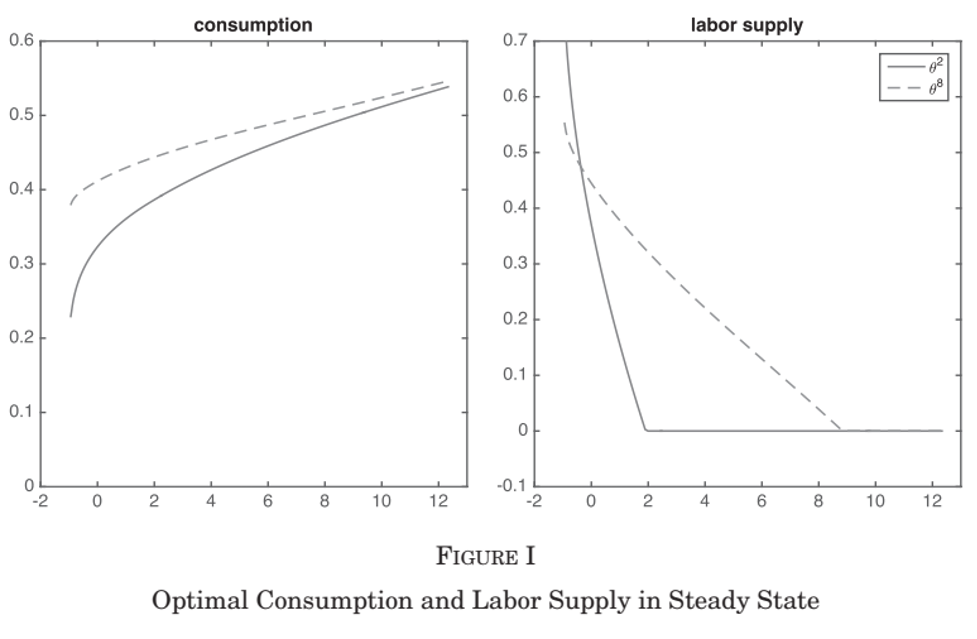
\includegraphics[width=6in]{Figures/Figure5.png}}
\label{fig:Figure5}

\caption{Optimal Consumption and Labor Supply in Steady State}
\end{figure}
The figures produced in our code closely resemble those found in the paper. The only notable difference is the labor supply function when $ \theta_{it} = \theta^{8}$.

\subsection{Optimal Consumption and Labor Supply for All $\theta_{it}$}
See Figure \ref{fig:Figure3} and Figure \ref{fig:Figure4}

\begin{figure}[h]
\centerline{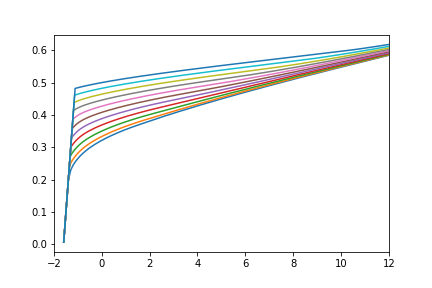
\includegraphics[width=6in]{Figures/Figure3.png}}
\label{fig:Figure3}
\caption{Optimal Consumption for All $\theta_{it}$}
\centerline{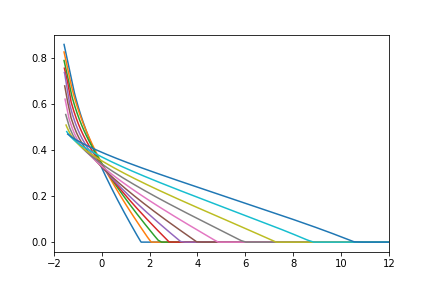
\includegraphics[width=6in]{Figures/Figure4.png}}
\label{fig:Figure4}
\caption{Optimal Labor Supply for All $\theta_{it}$}
\end{figure}


\clearpage\vfill\eject

\onlyinsubfile{\bibliography{\econtexRoot/GL2017}}

\end{document}
